\documentclass[12pt,a4paper,notitlepage]{report}
\usepackage[utf8]{inputenc}
\usepackage[czech]{babel}
\usepackage[pdftex]{graphicx} %pro vkládání obrázků v eps
\usepackage{hyperref} %pro kliknutelné linky
\usepackage[small,bf,belowskip=0.2cm]{caption} %změna stylu popisku a mezery před a za
\usepackage{sectsty} % pro jednoduché přestylování nadpisů
\usepackage{booktabs} % kvuli siunitx v tabulkach
\usepackage{array} %siunitx a centrovani tabulek
\usepackage{enumitem} %pro umravnění mezer v enumerate + změnu popisků
\usepackage{subcaption} %jako subfig ale muze mit refy v popiscich!!!
    %\renewcommand{\topfraction}{0.9}	% max fraction of floats at top
    %\renewcommand{\bottomfraction}{0.9}	% max fraction of floats at bottom
    
\hypersetup{
    pdfauthor={Tomáš Antecký},     % author
    pdftitle={Vliv modelu pro koeficient odporu na CFD simulaci suspendace v~mechanicky míchané nádobě},    % title
}   

%pro zdrojaky
\usepackage{listingsutf8}
\lstset{language=C,basicstyle=\footnotesize,numbers=left,showspaces=false,showstringspaces=false,numberstyle=\footnotesize,frame=single,title=\lstname,breaklines=true,inputencoding=utf8/latin2
} 

\usepackage[round]{natbib}
\usepackage{tabularx}
\usepackage{siunitx} %pro sazbu fyzikálních jednotek
\usepackage[top=2.5cm, bottom=2.5cm, left=2.5cm, right=2cm]{geometry} %nastaveni okraju a vzdalenosti cislovani

%pro vertikalni mezery u nadpisu
\usepackage[compact]{titlesec}
\titlespacing{\section}{0pt}{*3}{*0} %před a za
\titlespacing{\subsection}{0pt}{*3}{*0}
%\titlespacing{\subsubsection}{0pt}{*1}{*0}

\setlength{\textfloatsep}{0cm} %mezera za tabulkami


%nastaveni zobrazovani cisel jak je u nas zvykem :)
\sisetup{output-decimal-marker={,},exponent-product = \cdot, list-final-separator = { a }  }

%vypne vypisovani Kapitola u \chapter
\makeatletter
\def\@makechapterhead#1{%
  \vspace*{\p@}%
  {\parindent \z@ \raggedright \normalfont
    \interlinepenalty\@M
     \fontsize{17pt}{1}\selectfont \bfseries \thechapter\ \hspace{10pt} #1\par\nobreak
    \vskip 10\p@
  }}
\makeatother{}

%aby stejne vypadala i chapter*
\makeatletter
\def\@makeschapterhead#1{%
  \vspace*{\p@}%
  {\parindent \z@ \raggedright \normalfont
    \interlinepenalty\@M
     \fontsize{17pt}{1}\selectfont \bfseries #1\par\nobreak
    \vskip 10\p@
  }}
\makeatother{}

%chapter ted nedelani \newpage + pridana vspace
\makeatletter
\renewcommand\chapter{\vspace{0.7cm}\par%
  \thispagestyle{plain}%
  \global\@topnum\z@
  \@afterindentfalse
  \secdef\@chapter\@schapter}
\makeatother
{}

%velikost nadpisu
\sectionfont{\vspace{2mm}\fontsize{14pt}{1}\selectfont}
\subsectionfont{\vspace{2mm}\fontsize{12pt}{1}\selectfont}

%vlastni prikazy
\newcommand{\flu}{Ansys Fluent}

\addtocontents{toc}{\protect\thispagestyle{empty}} %odstraní číslování na stránce obsahu
\setcounter{tocdepth}{1}

\begin{document}
    \abovedisplayshortskip=-12pt %vertikální mezera před rovnicí
    %\belowdisplayshortskip=8pt  %vertikální mezera za rovnicí
    
    \abovedisplayskip=-10pt %vertikální mezera před rovnicí \noindent
    %\belowdisplayskip=0pt
	
	\pagestyle{empty} 
	\selectlanguage{czech}
	\begin{center}
{\Large VYSOKÁ ŠKOLA CHEMICKO-TECHNOLOGICKÁ V PRAZE\\}
{\large Fakulta chemicko-inženýrská\\
\textbf{Ústav chemického inženýrství}\\}
\vspace{15mm}

\begin{figure}[!h]
\begin{center}
\includegraphics[angle=0,width=27mm]{images/logo_vscht.eps}
\end{center}
\end{figure}

\vspace{25mm}

{\huge \textbf{CFD simulace\\}}
\vspace{10mm}
{\Large \textbf{SVK 2011\\}}
\end{center}
\vspace{35mm}

%\null
%\vfill

\begin{tabular}{p{50mm}lp{50mm}}
Vypracoval: & \textbf{Bc.\,Tomáš Antecký}\\
\\
Vedoucí práce: & Doc.\,Dr.\,Ing.\,Milan Jahoda \\

\\
Studijní program: & Procesní inženýrství a informatika \\
\\
Studijní obor: & Chemické inženýrství, bioinženýrství \\
	& a matematické modelování procesů\\
\end{tabular}

  \section*{Souhrn}
\vspace{3mm}
Naplní práce byla studie suspendace pevné fáze v mechanicky míchané nádobě pomocí počítačové dynamiky tekutin. Práce se především zaměřuje na různé možnosti popisu mezifázové odporové síly, která významným způsobem ovlivňuje kvalitu výsledné vícefázové simulace. Bylo vyzkoušeno několik korelací pro koeficient odporu vyvinutých pro turbulentní oblast proudění. Zmíněné modely však nejsou dostupné v použitém simulačním softwaru ANSYS FLUENT, a proto byly v rámci studie implementovány v podobně uživatelsky definovaných funkcí. Na závěr byly představeny a porovnány dosavadní výsledky získané pomocí CFD simulace pro odlišně zvolené korelace koeficientu odporu.

	\tableofcontents{}
	\pagestyle{plain}
  \newpage
  \setlength{\baselineskip}{1.5\baselineskip}
	\setcounter{page}{1}
	
  \input{uvod}
  \chapter{Teoretická část}



\section{Počítačová dynamika tekutin}

\section{Vícefázové modely}
V současnosti existuje řada matematických modelů, které popisují vícefázové proudění. Následující kapitola obsahuje přehled modelů, které jsou vhodné k simulaci suspendace v mechanicky míchaných nádobách.

\subsection{Eulerian-Lagrangian}
Tento typ modelu uvažuje primární tekutou fází jako kontinuum s dispergovanou sekundární fází. Pro primární fázi je řešena rovnice kontinuity spolu s Navierovými-Stokesovými rovnicemi, zatímco pro dispergovanou fázi je řešena trajektorie každé částice separátně. Jednotlivé fáze si mohou mezi sebou vyměňovat hmotu, hybnost a energii, avšak vzájemné interakce částic nebo jejich rozpad jsou zanedbány. Model Eulerian-Lagrangian je především vhodný pro systémy, kde objemový zlomek dispergované fáze nepřesáhne \SI{10}{\percent} např: rozprašovací sušárny, cyklóny nebo spalování uhlí či kapalného paliva. 

Řešením bilance sil působící na částici (rov. \ref{eq:dpm}) je získána její trajektorie v daném časovém okamžiku.

\begin{equation}
	\frac{d\vec{v}_{p}}{dt} = \vec{F}_{D}(\vec{v}_{f} - \vec{v}_{p}) + \frac{\vec{g}(\rho_{p} - \rho_{f})}{\rho_{p}} + \frac{\vec{F}_{ad}}{\rho_{p}}
	\label{eq:dpm}
\end{equation} 

\noindent Kde jednotlivé členy značí:

\begin{itemize}[itemsep=0pt,parsep=0pt,partopsep=0pt,topsep=0pt]
  \item $\vec{v}_{p}$ vektor rychlosti dané částice
  \item $\vec{v}_{f}$ vektor rychlosti tekutiny
  \item $\rho_{p}$, $\rho_{f}$ hustotu částice resp. tekutiny
  \item $\vec{g}$ gravitační zrychlení
  \item $\vec{F}_{D}$ odporová síla
  \item $\vec{F}_{ad}$ další síly (např: tlaková, zdánlivá síla, síla zahrnující vliv rotace atd.)
\end{itemize}

\subsection{Eulerian-Eulerian}
U modelu Eulerian-Eulerian jsou jednotlivé fáze považovány za prostupující se kontinua a každý bod v systému obsahuje informaci o objemovém zlomku dané fáze. Z tohoto popisu je zřejmé, že suma objemových zlomků přes všechny fáze v libovolném bodě se vždy musí rovnat jedné. 

\begin{equation}
	\sum_{i=1}^n \alpha_{i} = 1
	\label{eq:volfrac}
\end{equation} 

\noindent Jednotlivé fáze mohou být kapalné, plynné nebo pevné a jejich celkový počet není teoreticky limitován. Pro každou fázi se řeší rovnice kontinuity a sada momentových (Navierových-Stokesových) rovnic a k výměně hybnosti mezi jednotlivými fázemi slouží mezifázové členy v těchto rovnicích. Pokud dochází k přenosu tepla nebo hmoty je třeba tuto skutečnost zohlednit v bilanci energie a hmoty.    

Pokud nedochází k výměně hmoty mezi jednotnými fázemi tak rovnice kontinuity pro $i$-tou fázi má tvar:

\begin{equation}
	\frac{\partial}{\partial t} (\alpha_{i}\rho_{i}) +  \nabla \cdot (\alpha_{i}\rho_{i}\vec{v}_{i}) = 0
	\label{eq:conti}
\end{equation}

\noindent Momentovou rovnici pro $i$-tou fázi za stejných předpokladů lze zapsat jako:

\begin{equation}
	\frac{\partial}{\partial t} (\alpha_{i}\rho_{i}\vec{v}_{i}) + \nabla \cdot (\alpha_{i}\rho_{i} \vec{v}_{i} \otimes \vec{v}_{i}) = -\alpha_{i} \nabla p + \nabla \cdot \bar{\tau} + \alpha_{i}\rho_{i}\vec{g} + \sum_{j=1}^n \vec{R}_{ji} + \vec{F}_{ext} + \vec{F}_{int}
	\label{eq:conti}
\end{equation}

\noindent kde $p$ je tlak, $\bar{\tau}$ je tenzor napětí, jehož konkretní tvar závisí na typu uvažované fáze. Člen $\vec{R}_{ji}$ představuje mezifázovou odporovou sílu, $\vec{F}_{ext}$ má význam vnější objemové síly a $\vec{F}_{int}$ zahrnuje 

\subsection{Eulerian-Granular}


  \chapter{Experimentální část}
Experimentální studii suspendace v mechanicky míchané nádobě provedla Bc.\,Zuzana Pavlíková v rámci své bakalářské práce na Ústavu chemického inženýrství VŠCHT Praha v roce 2011.

\section{Popis experimentu}
Náplní experimentu bylo měření průběhu homogenizace kapaliny v přítomnosti pevné fáze a následném zjišťování doby homogenizace. K provedení experimentu byla využita válcová nádoba z plexiskla o vnitřním průměru $T=\SI{0.29}{\meter}$ s plochým dnem, jenž byla opatřena čtyřmi radiálními narážkami o šířce $b=T/10$. Výška plnění nádoby byla zvolena $H=T$. 

\begin{figure}[h!]
\begin{center}
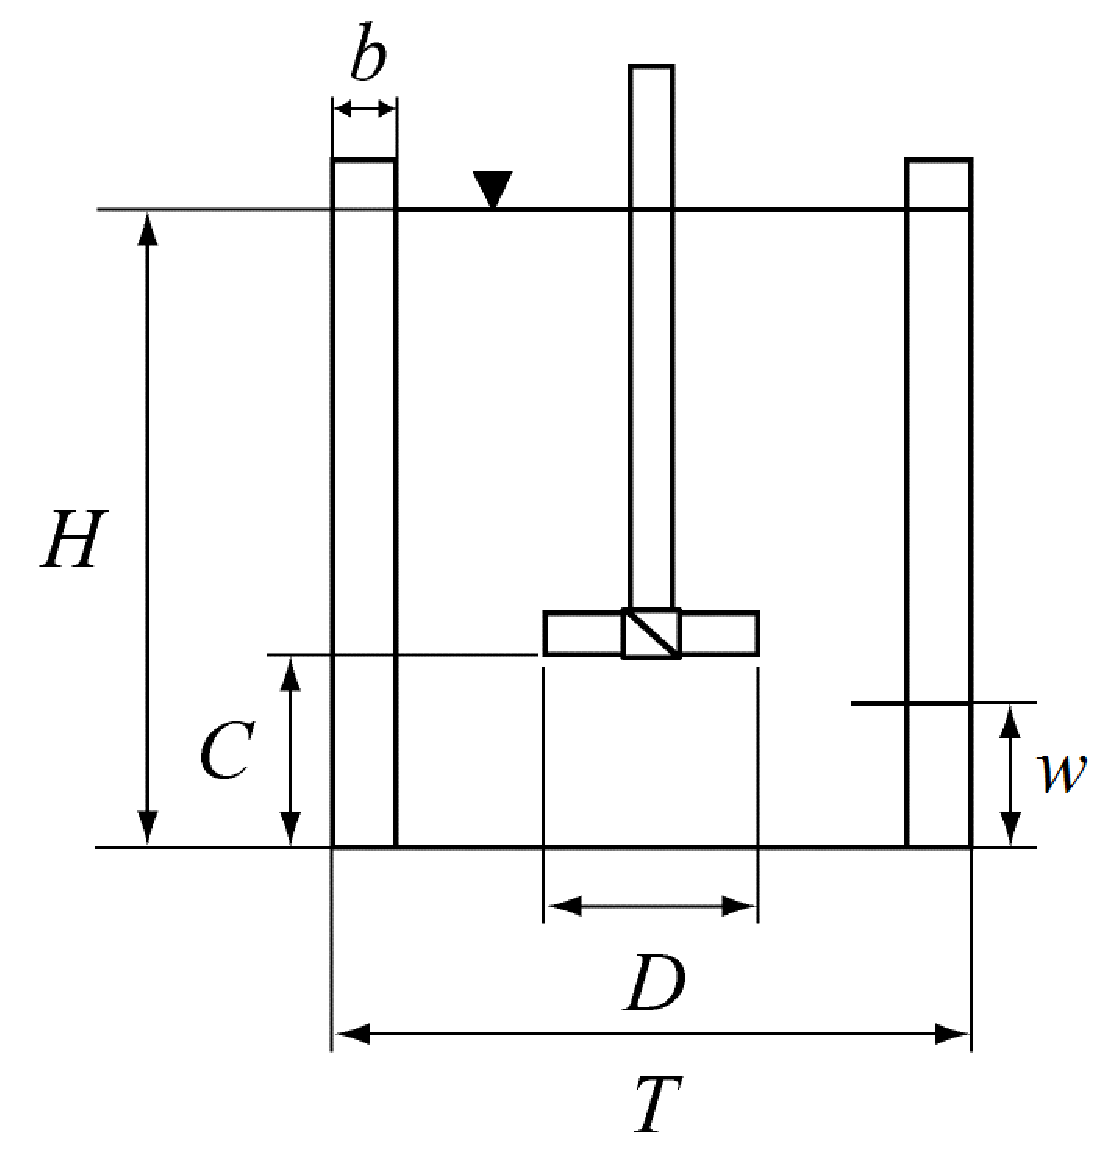
\includegraphics[scale=0.45]{images/mujedit.eps}
\caption{Geometrie experimentu}
\label{fig:nadoba}
\end{center}
\end{figure} 

Do nádoby $C=T/3$ ode dna bylo umístěno šestilopatkové míchadlo se šikmo skloněnými lopatkami (úhel zkosení \SI{45}{\degree}). Rychlost otáčení byla postupně volena  \SIlist[list-units = single]{3;4;5;6;7;8;9}{\per\second}. Celkový průměr míchadla činil $D=T/3$ a ostatní jeho rozměry jsou zobrazuje obr. XX.      

Jako vsádka byla použita voda a polyvinylpyrrolidon (PVP). Pevnou fázi tvořily červené kuličky z polyvinyl (PVC) o 

  
  \chapter{Výpočetní část}

\section{Tvorba geometrie}

Výpočetní doména byla vytvořena v programu Ansys DesignModeler podle geometrie uvedené v kapitole \ref{chap:exp}. Výsledná nestrukturovaná síť byla tvořena šestistěnnými a čtyřstěnnými buňkami o celkovém počtu \num{264398}. Průměrný objem buňky činil \SI{0.07}{\milli\litre} a průměrný skewness faktor \num{0.162}. Výpočetní doména je znázorněna na obr. \ref{fig:geo}, kde zelenou barvou je znázorněna rotační zóna kolem míchadla. 

\begin{figure}[h!]
\begin{center}
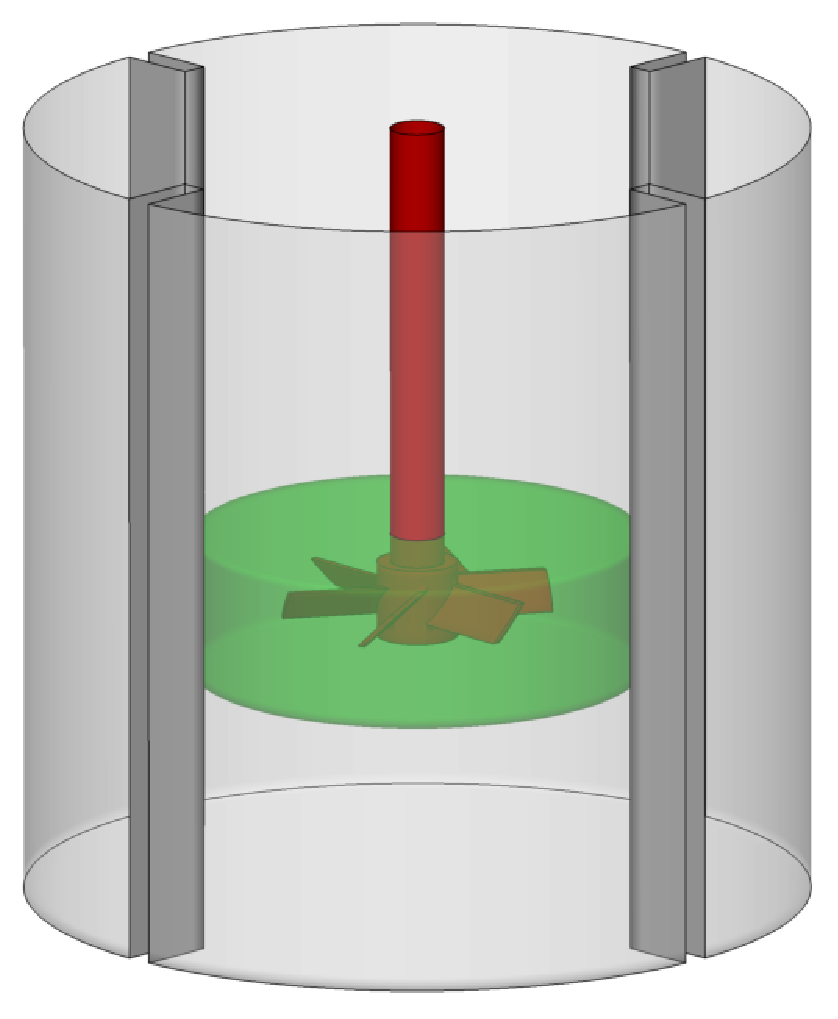
\includegraphics[scale=0.3]{images/geo.eps}
\caption{Výpočetní doména}
\label{fig:geo}
\end{center}
\end{figure} 

\section{Uživatelsky definové funkce}
Uživatelem definované funkce (UDF) jsou moduly načítané do softwaru \flu, jenž rozšiřují nebo upravují schopnosti řešiče. Například může se jednat o definovaní vlastních počátečních a okrajových podmínek, změnu materiálových vlastností a modifikaci simulačních modelů. Pro tvorbu zdrojových souborů se využívá programovací jazyk C, které jsou následně zkompilovaný do dynamické knihovny.

Všechny korelace pro odporový koeficient uvedené v tab. \ref{tab:cds} byly implementovány v podobě uživatelsky definovaných funkcí a jejich zdrojové kódy jsou uvedeny v kapitole Příloha.


  \chapter{Výsledková část}
Následující kapitola shrnuje získané výsledky pomocí CFD simulace popsané v předcházejících odstavcích. 

Na obr. \ref{fig:vecfield} je znázorněno vektorové pole rychlosti kapaliny v řezu nádobou a čase \SI{6}{\second}, což již lze považovat za poměrně ustálený stav. Z obrázku je dobře patrný vznikl sekundárních cirkulačních smyček v prostoru pod míchadlem. Tento jev byl experimentálně pozorován řadou autorů (např. \citet{hos10}) při zvolené světlé výšce míchadla od $C=T/2$ do $C=T/6$.  

\begin{figure}[h!]
\begin{center}
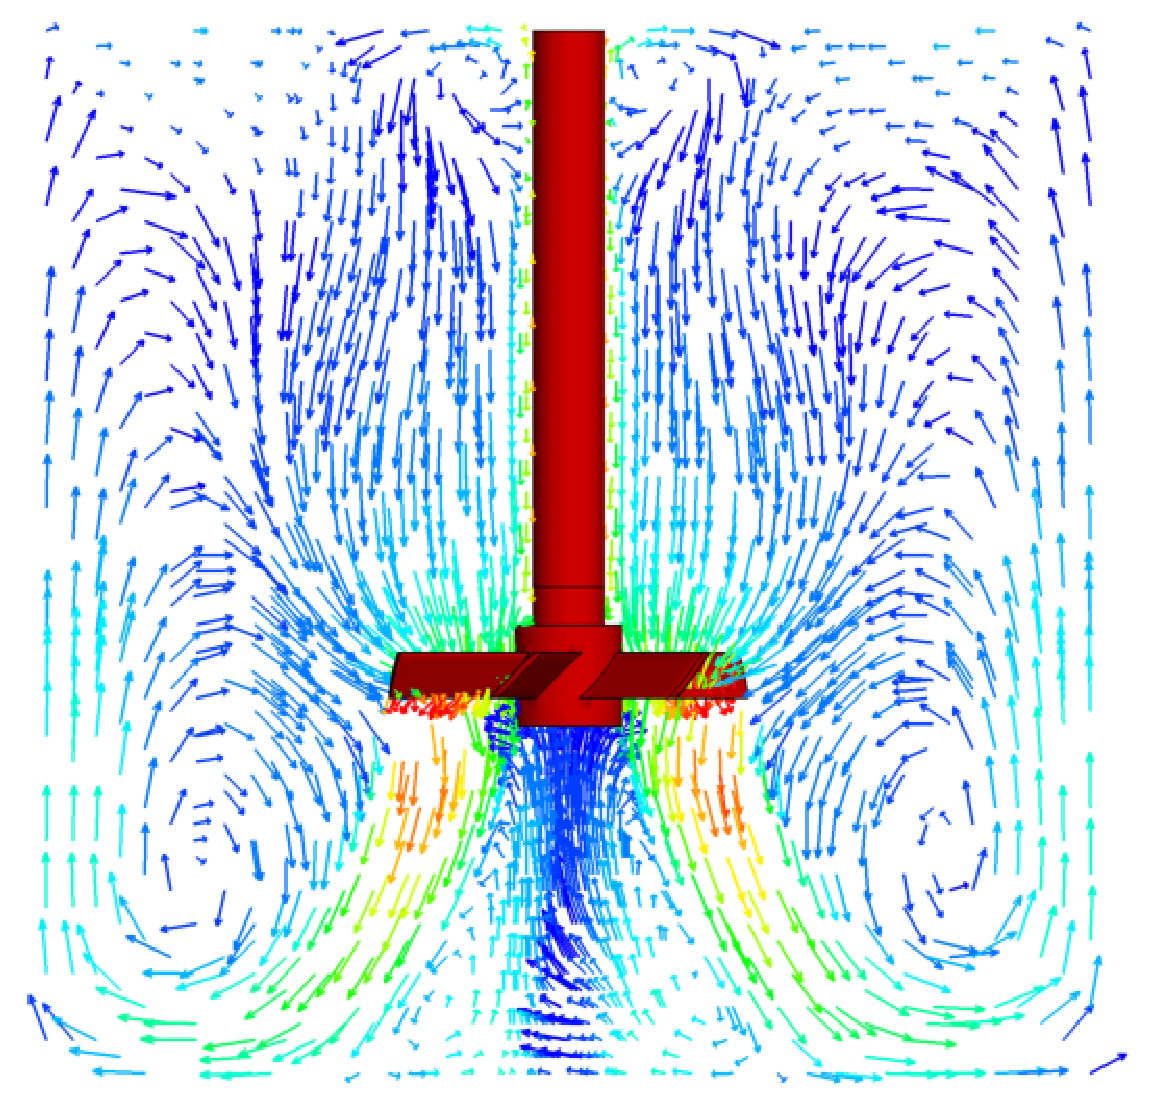
\includegraphics[scale=0.5]{images/vecfield.eps}
\caption{Vektorové pole rychlosti}
\label{fig:vecfield}
\end{center}
\end{figure} 

\vspace{-9mm}

Obr. \ref{fig:count2} zobrazuje kontury objemového zlomku pevné fáze v řezu míchací nádobou pro vybrané korelace odporového koeficientu. Tyto údaje byly získány v času simulace \SI{2}{\second}. Z obrázků je dobře patrné, že přímo pod míchadlem je největší koncentrace pevné fáze vlivem sekundárních cirkulačních smyček. Korelace odporového koeficientu podle Brucata v tomto případě předpovídá významně vyšší rozložení kuliček z PVC pod míchadlem než zbývající modely.

\newpage

\begin{figure}[h!]
  \begin{center}
  \subfloat[Schiller-Naumann]{\label{fig:neu2}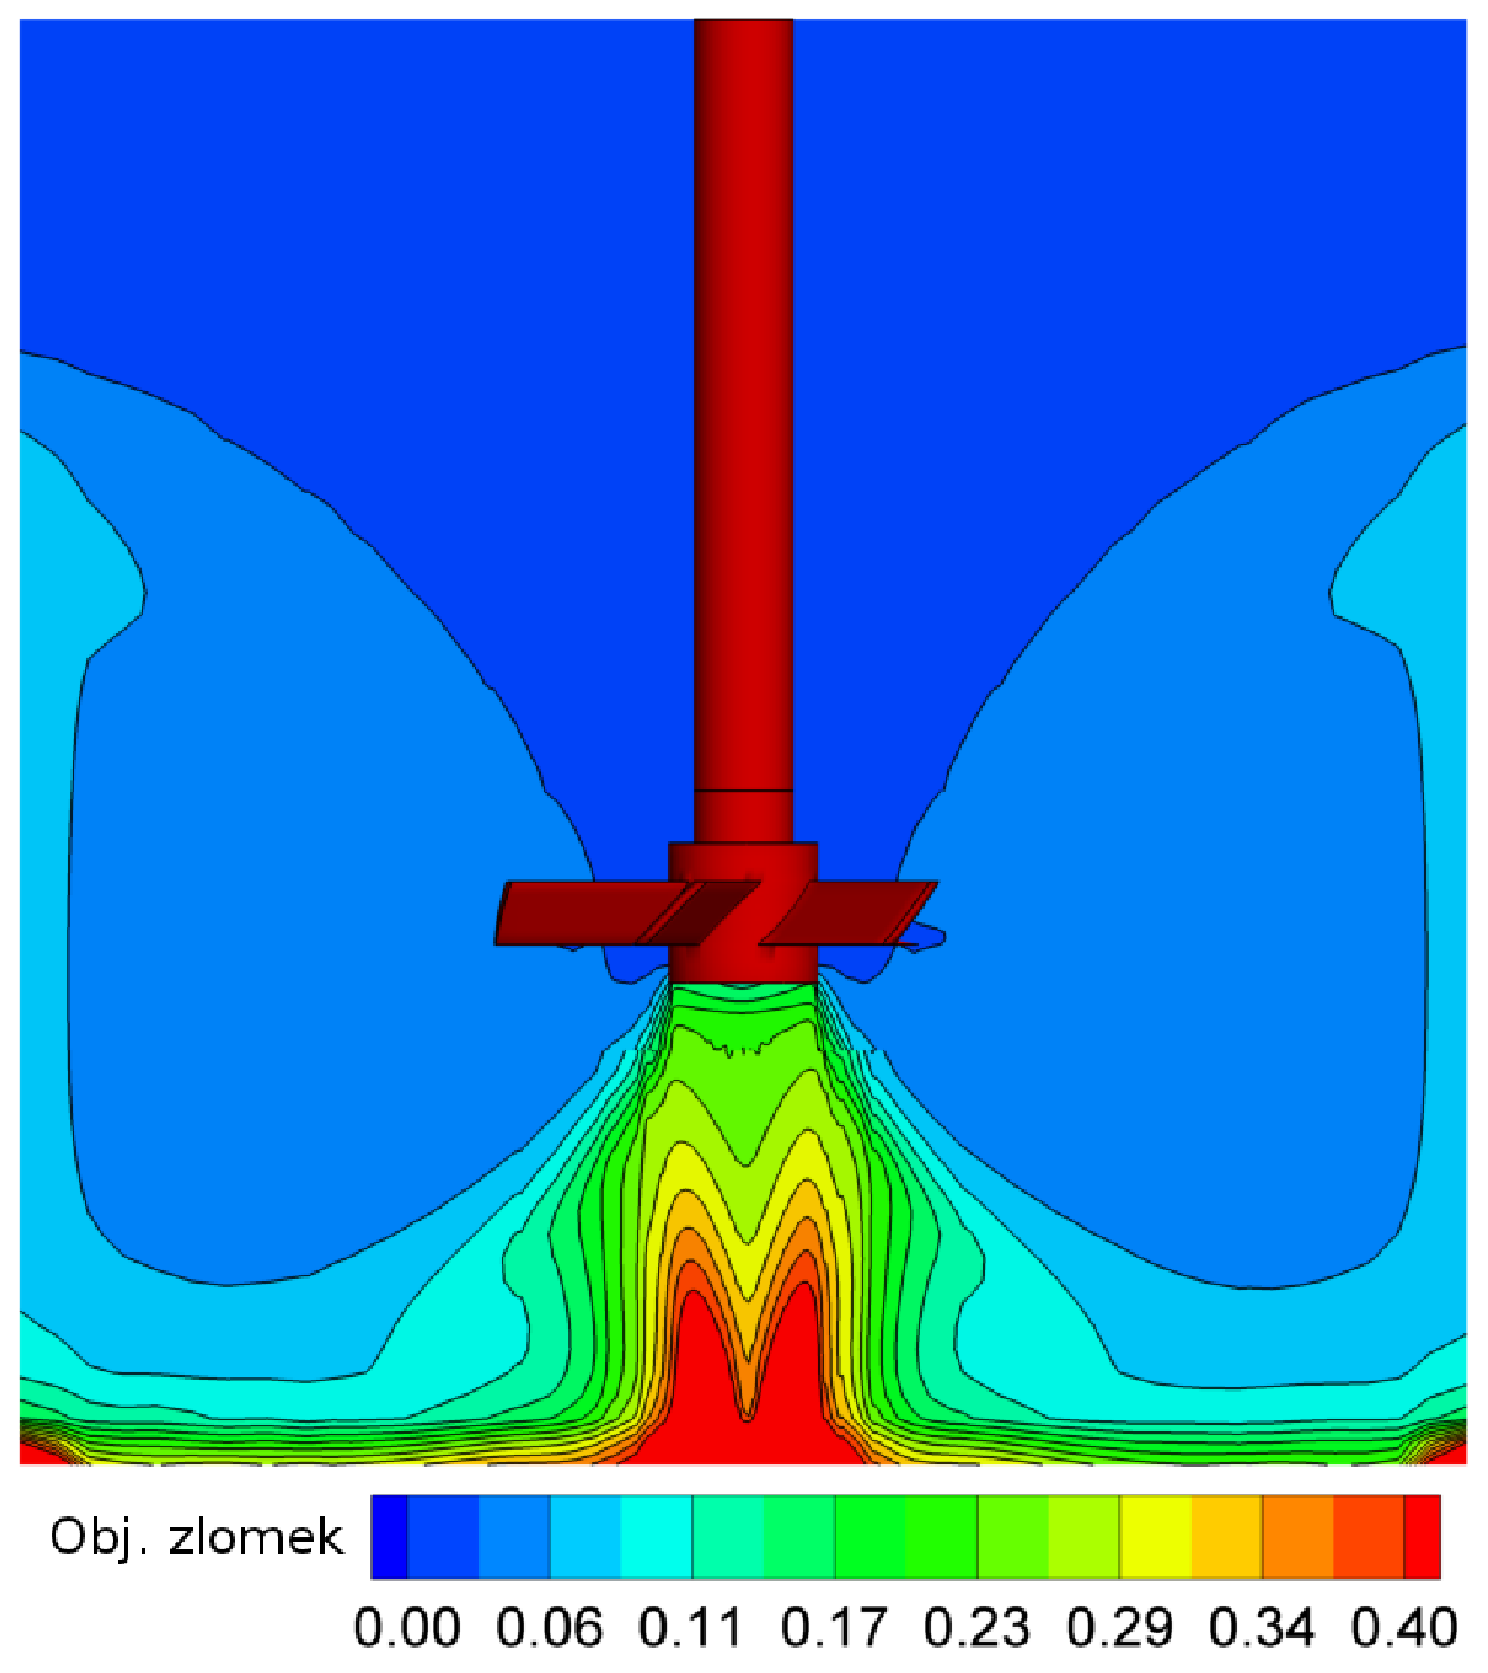
\includegraphics[scale=0.3]{images/volSch-2.eps}}  
  \qquad             
  \subfloat[Pinelli]{\label{fig:pin2}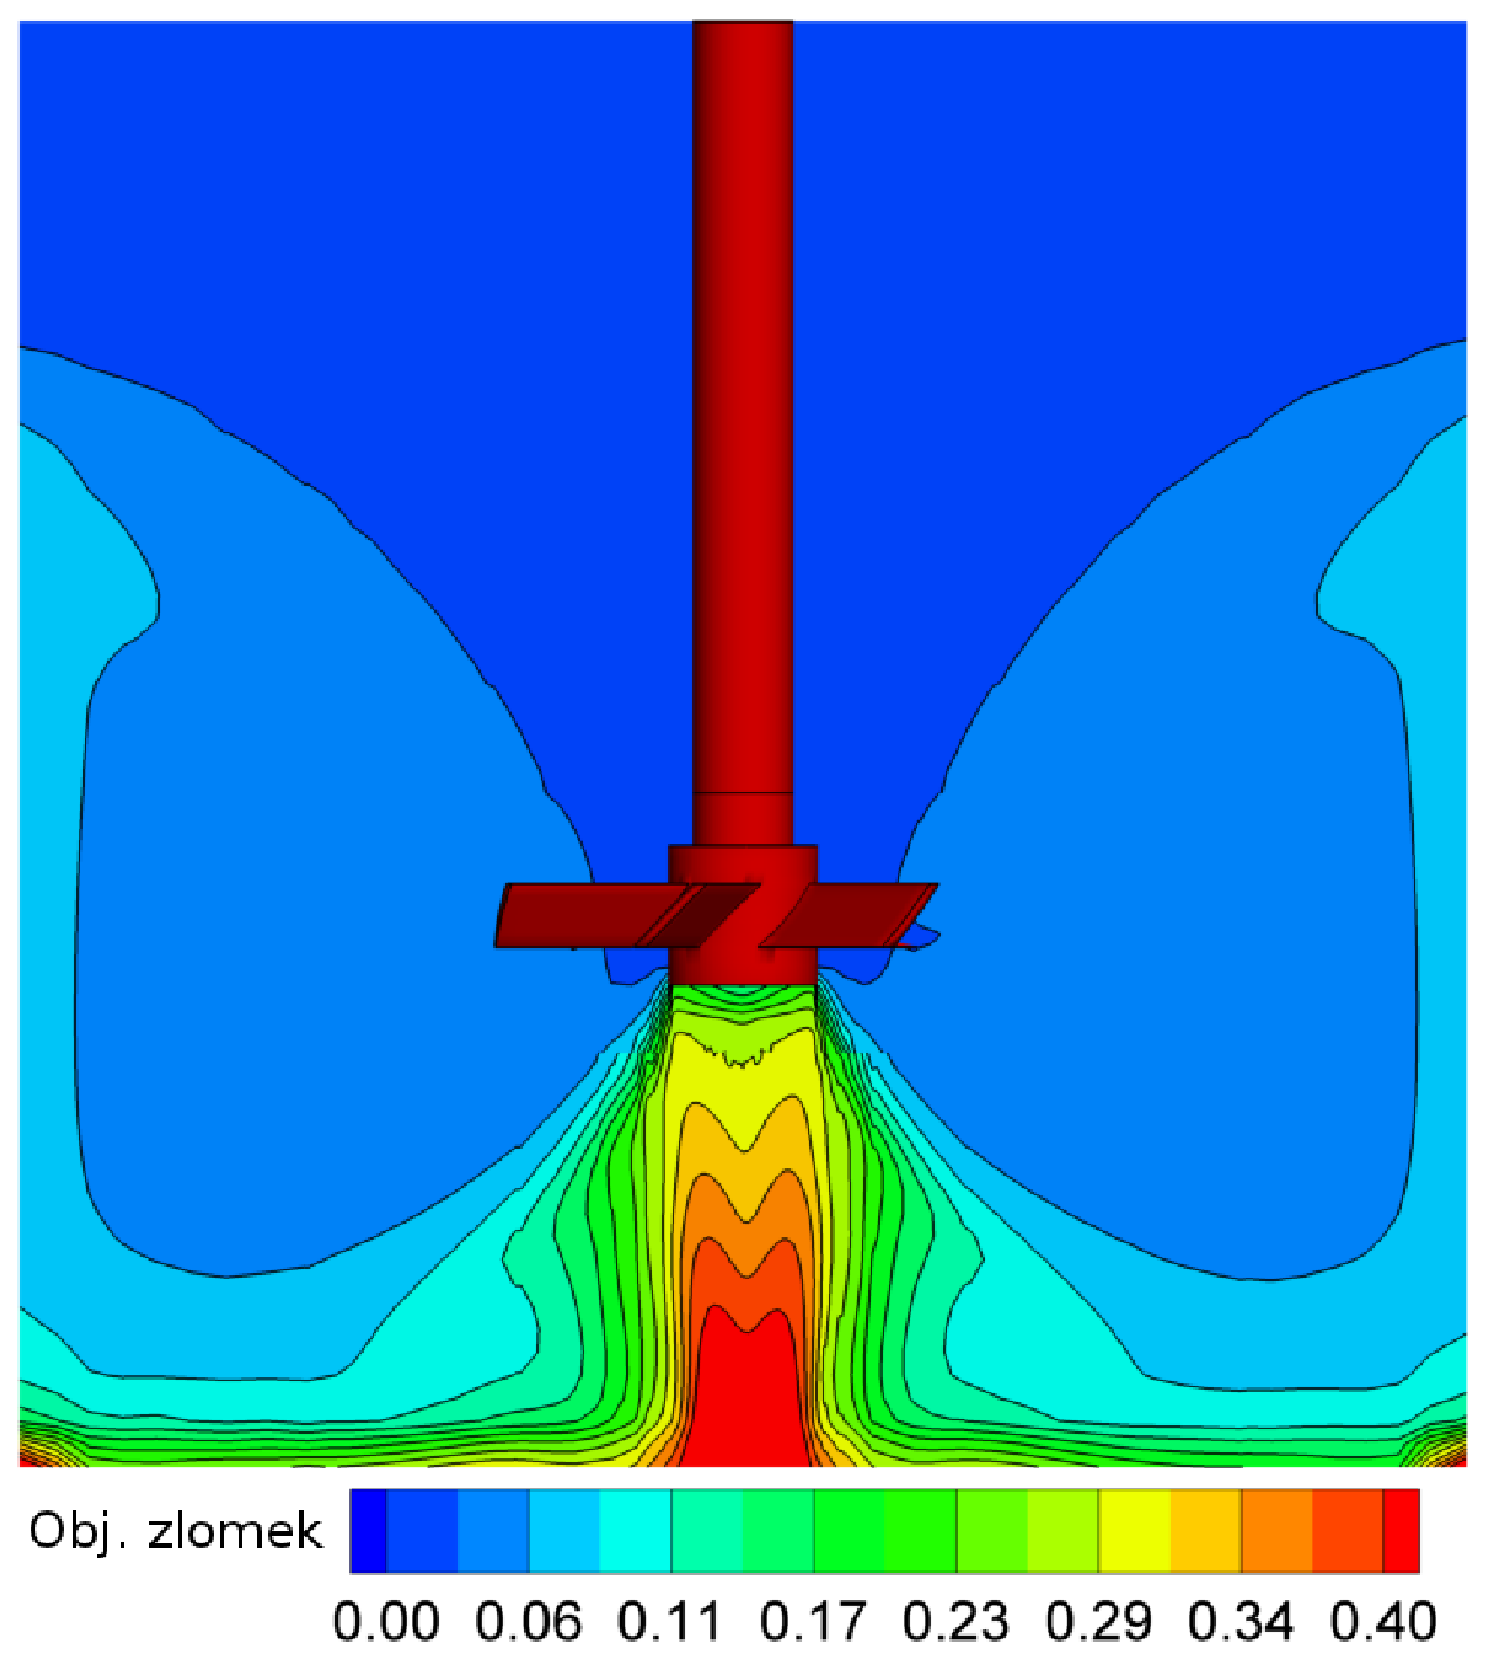
\includegraphics[scale=0.3]{images/volPin-2.eps}}
  \\
  \subfloat[Brucato]{\label{fig:bru2}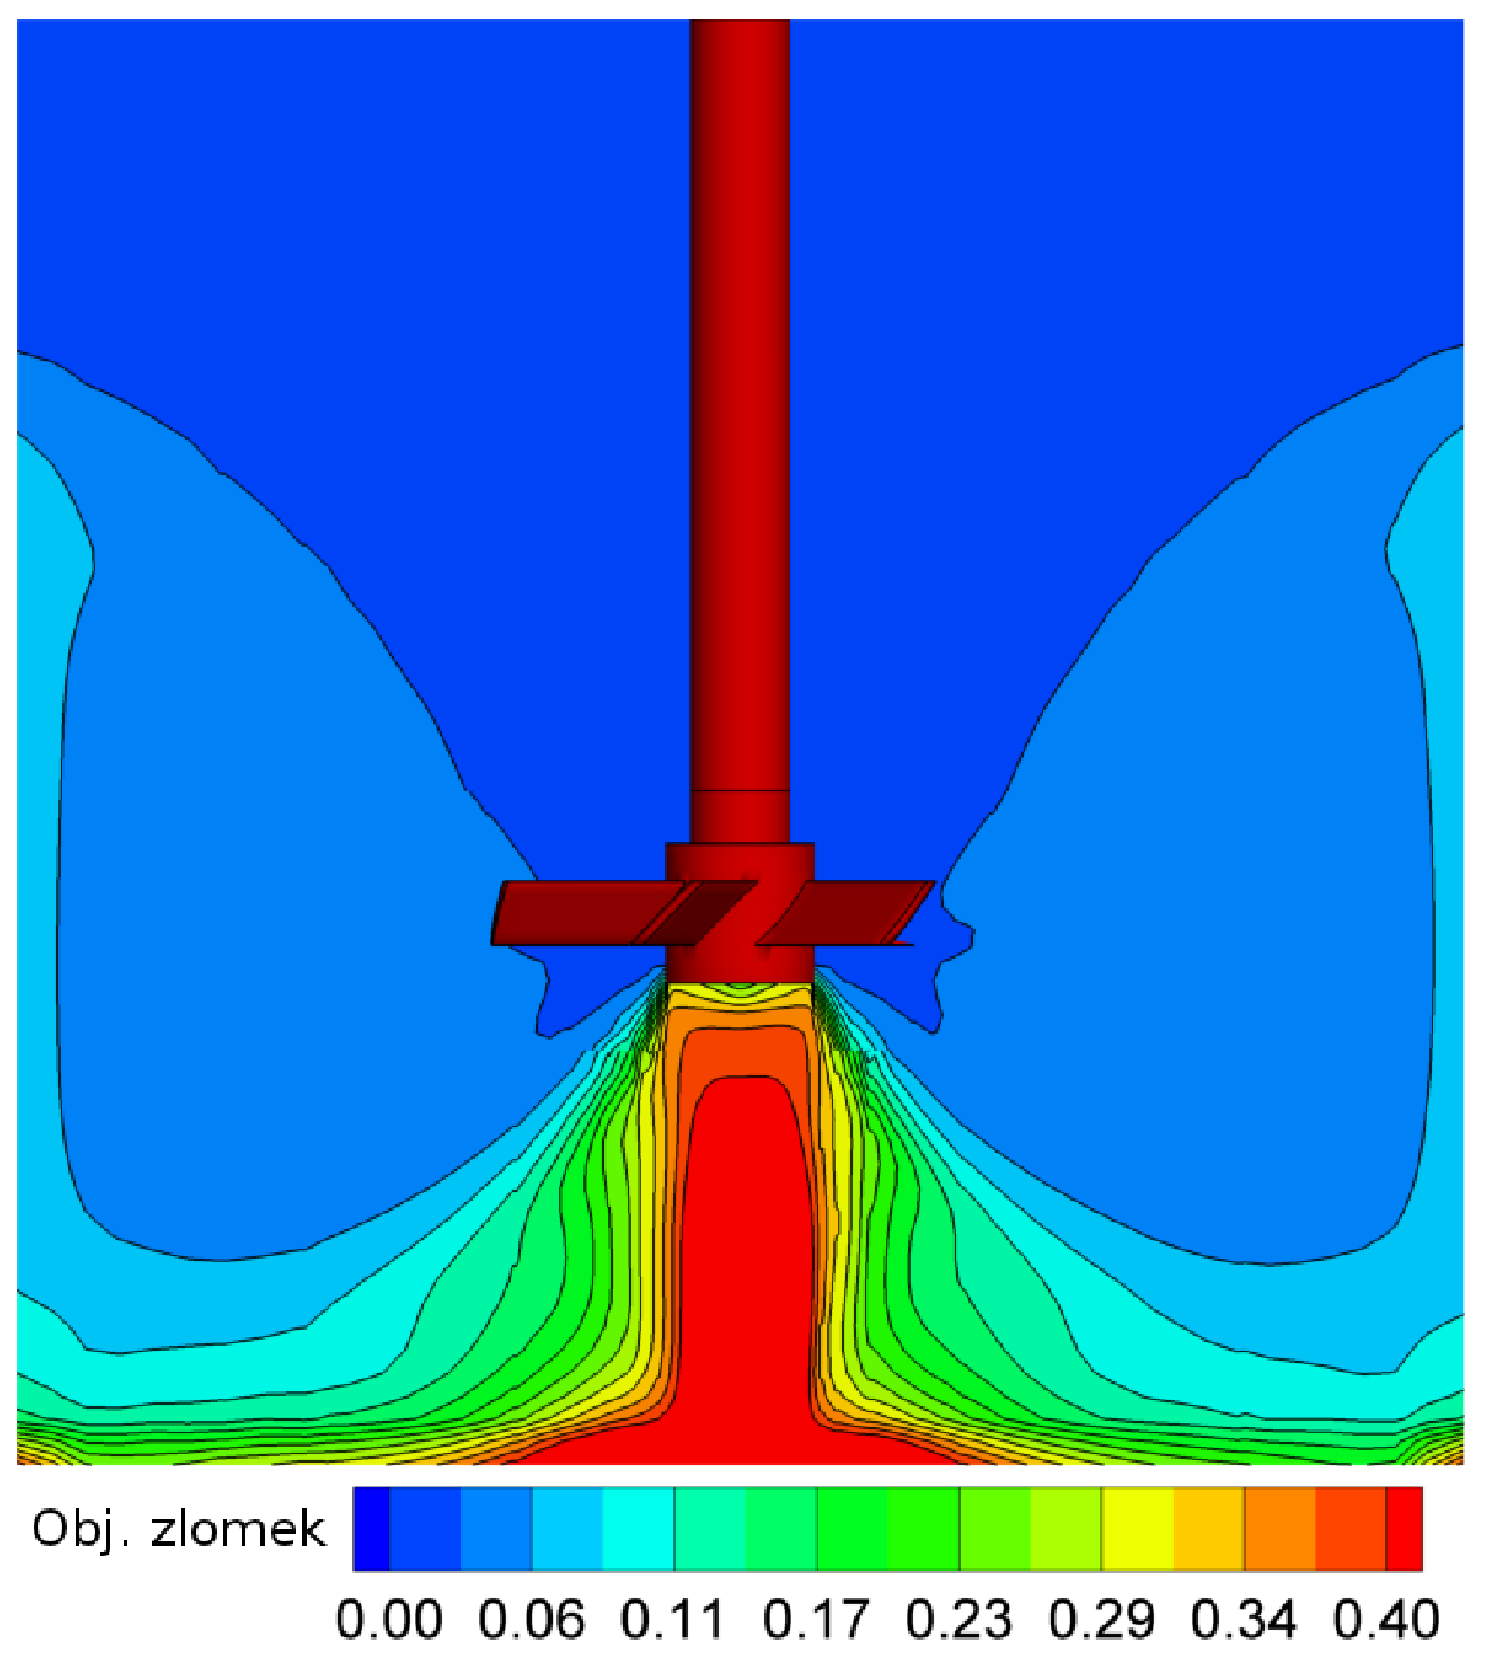
\includegraphics[scale=0.3]{images/volBru-2.eps}}
  \qquad
  \subfloat[Khopkar]{\label{fig:kho2}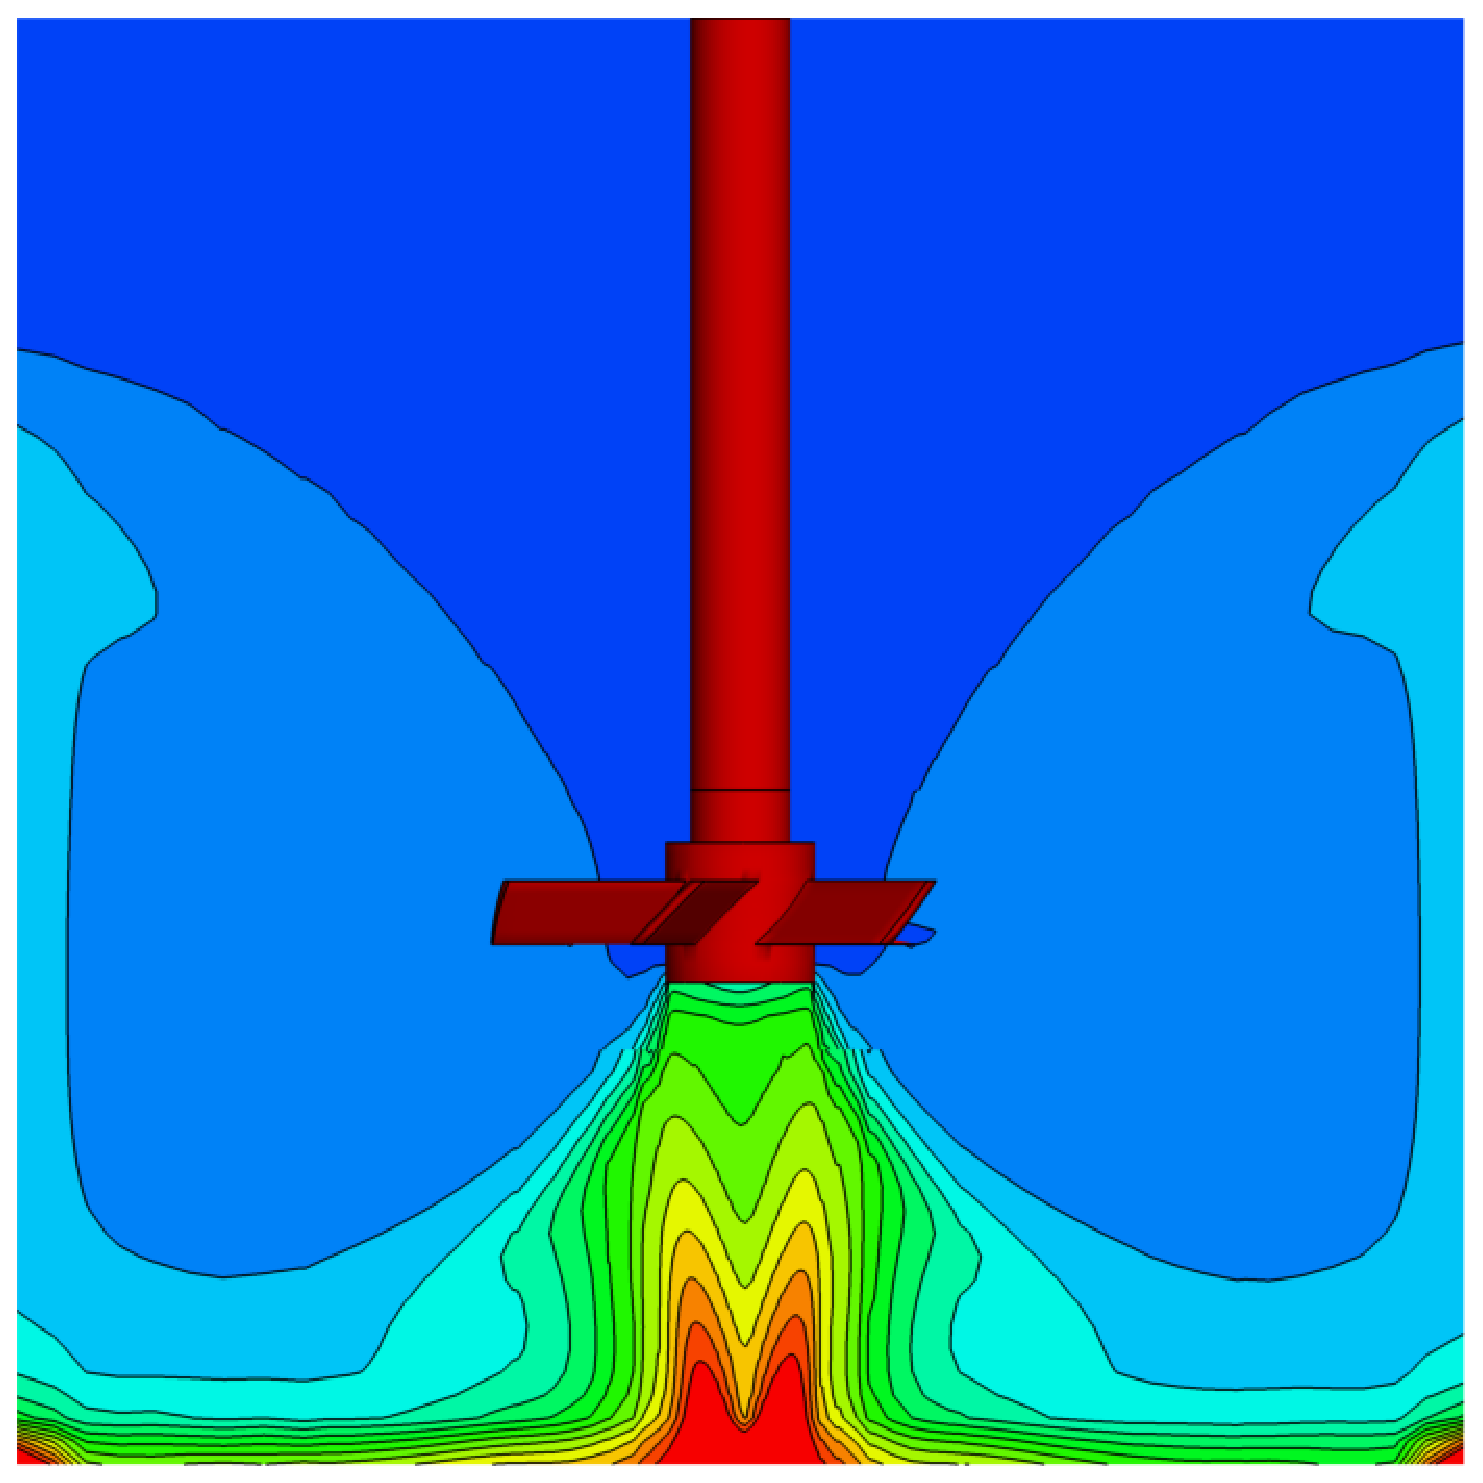
\includegraphics[scale=0.3]{images/volKho-2.eps}}
  \caption{Kocentrace pevné fáze v čase \SI{2}{\second}}
  \label{fig:count2}
  \end{center}
\end{figure}

\vspace{-9mm}

Následují opět obrázky zachycují objemový zlomek pevné fáze v řezu nádobou, avšak v tomto případě pro čas \SI{6}{\second}. Pevná fáze je již poměrně rozptýlena, ale stále se pod míchadlem nacházejí oblasti se zvýšenými koncentracemi.

\newpage

\begin{figure}[h!]
  \begin{center}
  \subfloat[Schiller-Naumann]{\label{fig:neu6}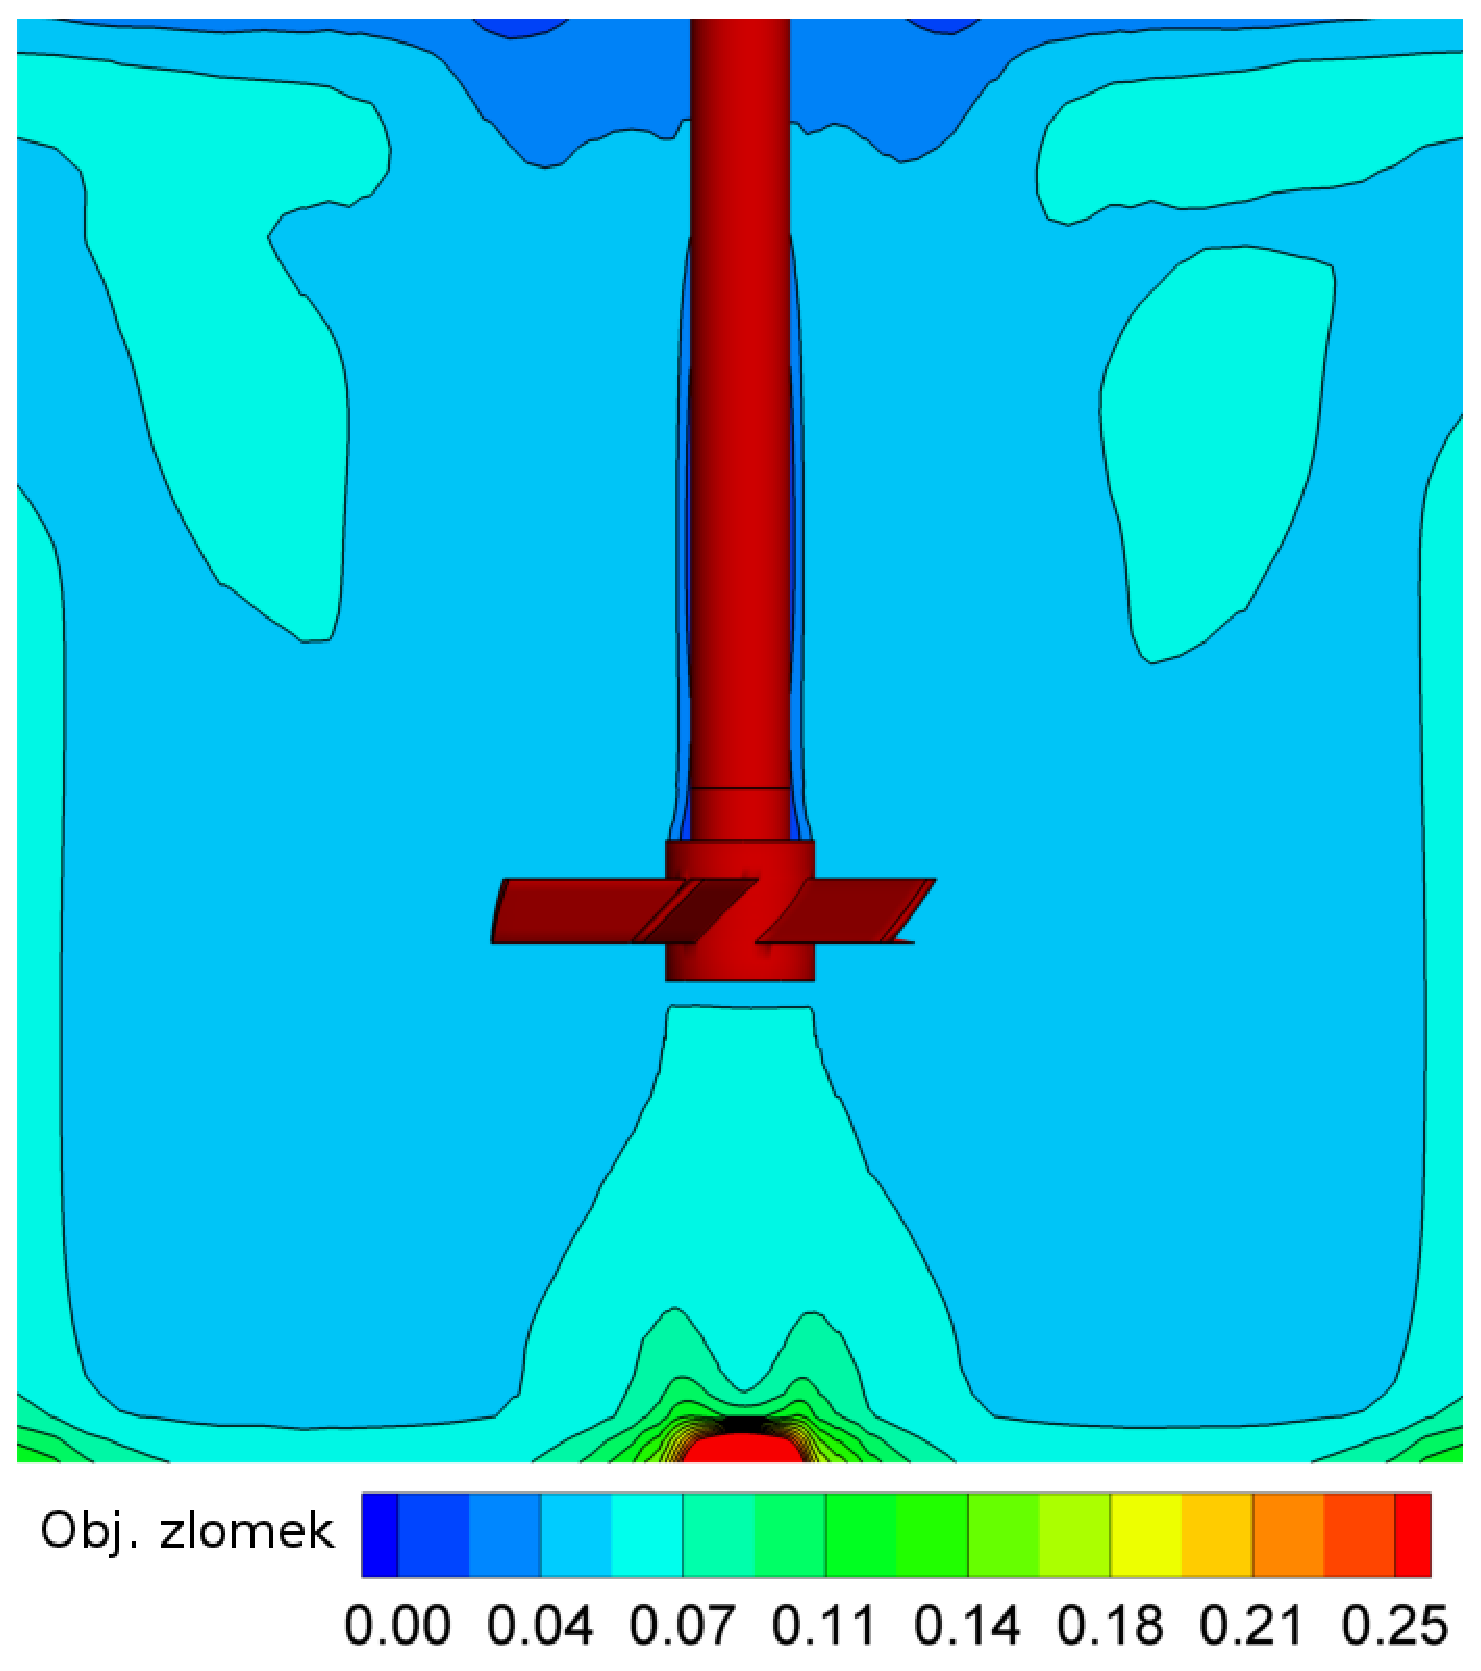
\includegraphics[scale=0.3]{images/volSch-6.eps}}  
  \qquad             
  \subfloat[Pinelli]{\label{fig:pin6}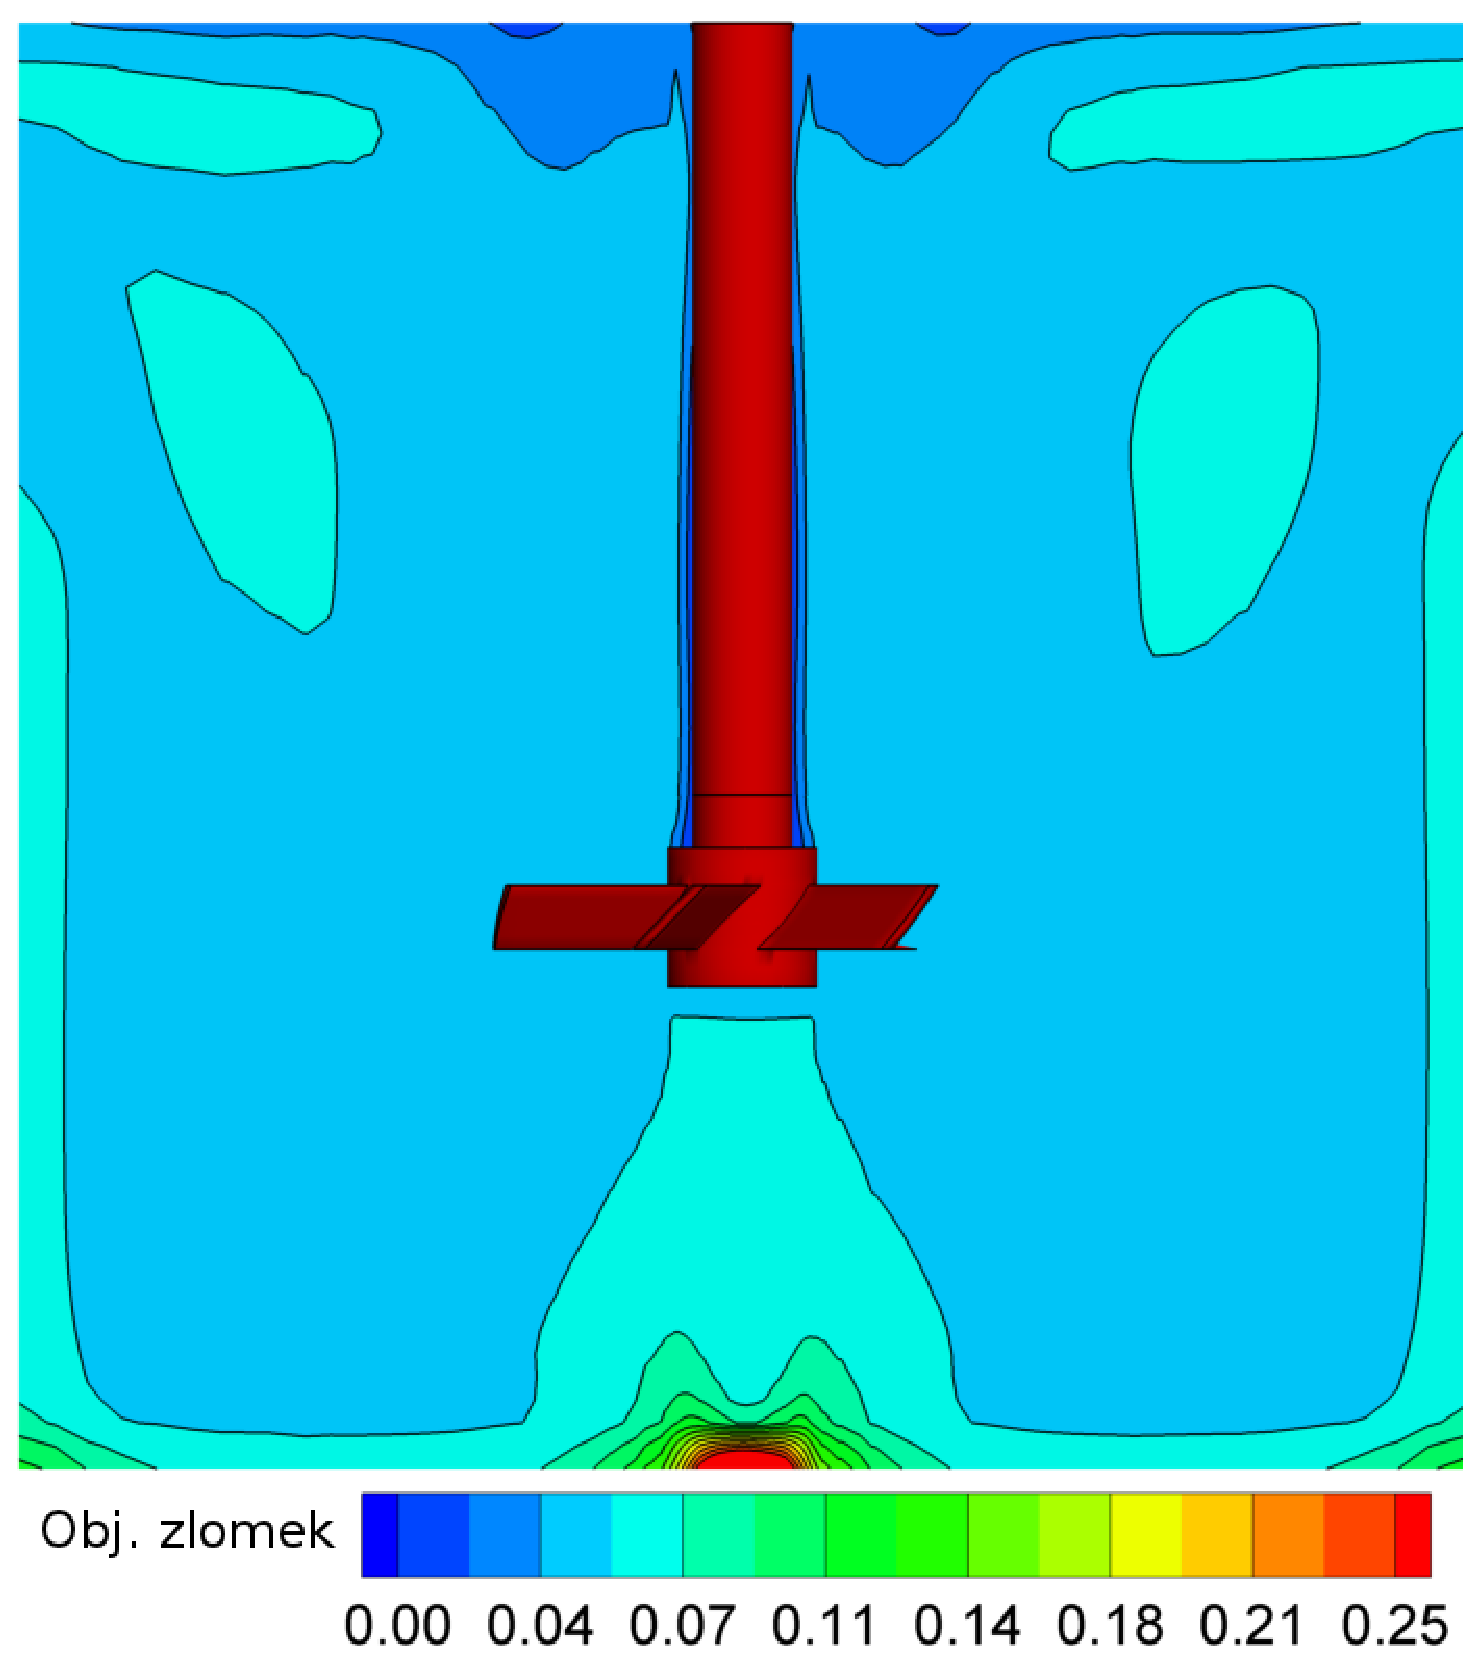
\includegraphics[scale=0.3]{images/volPin-6.eps}}
  \\
  \subfloat[Brucato]{\label{fig:bru6}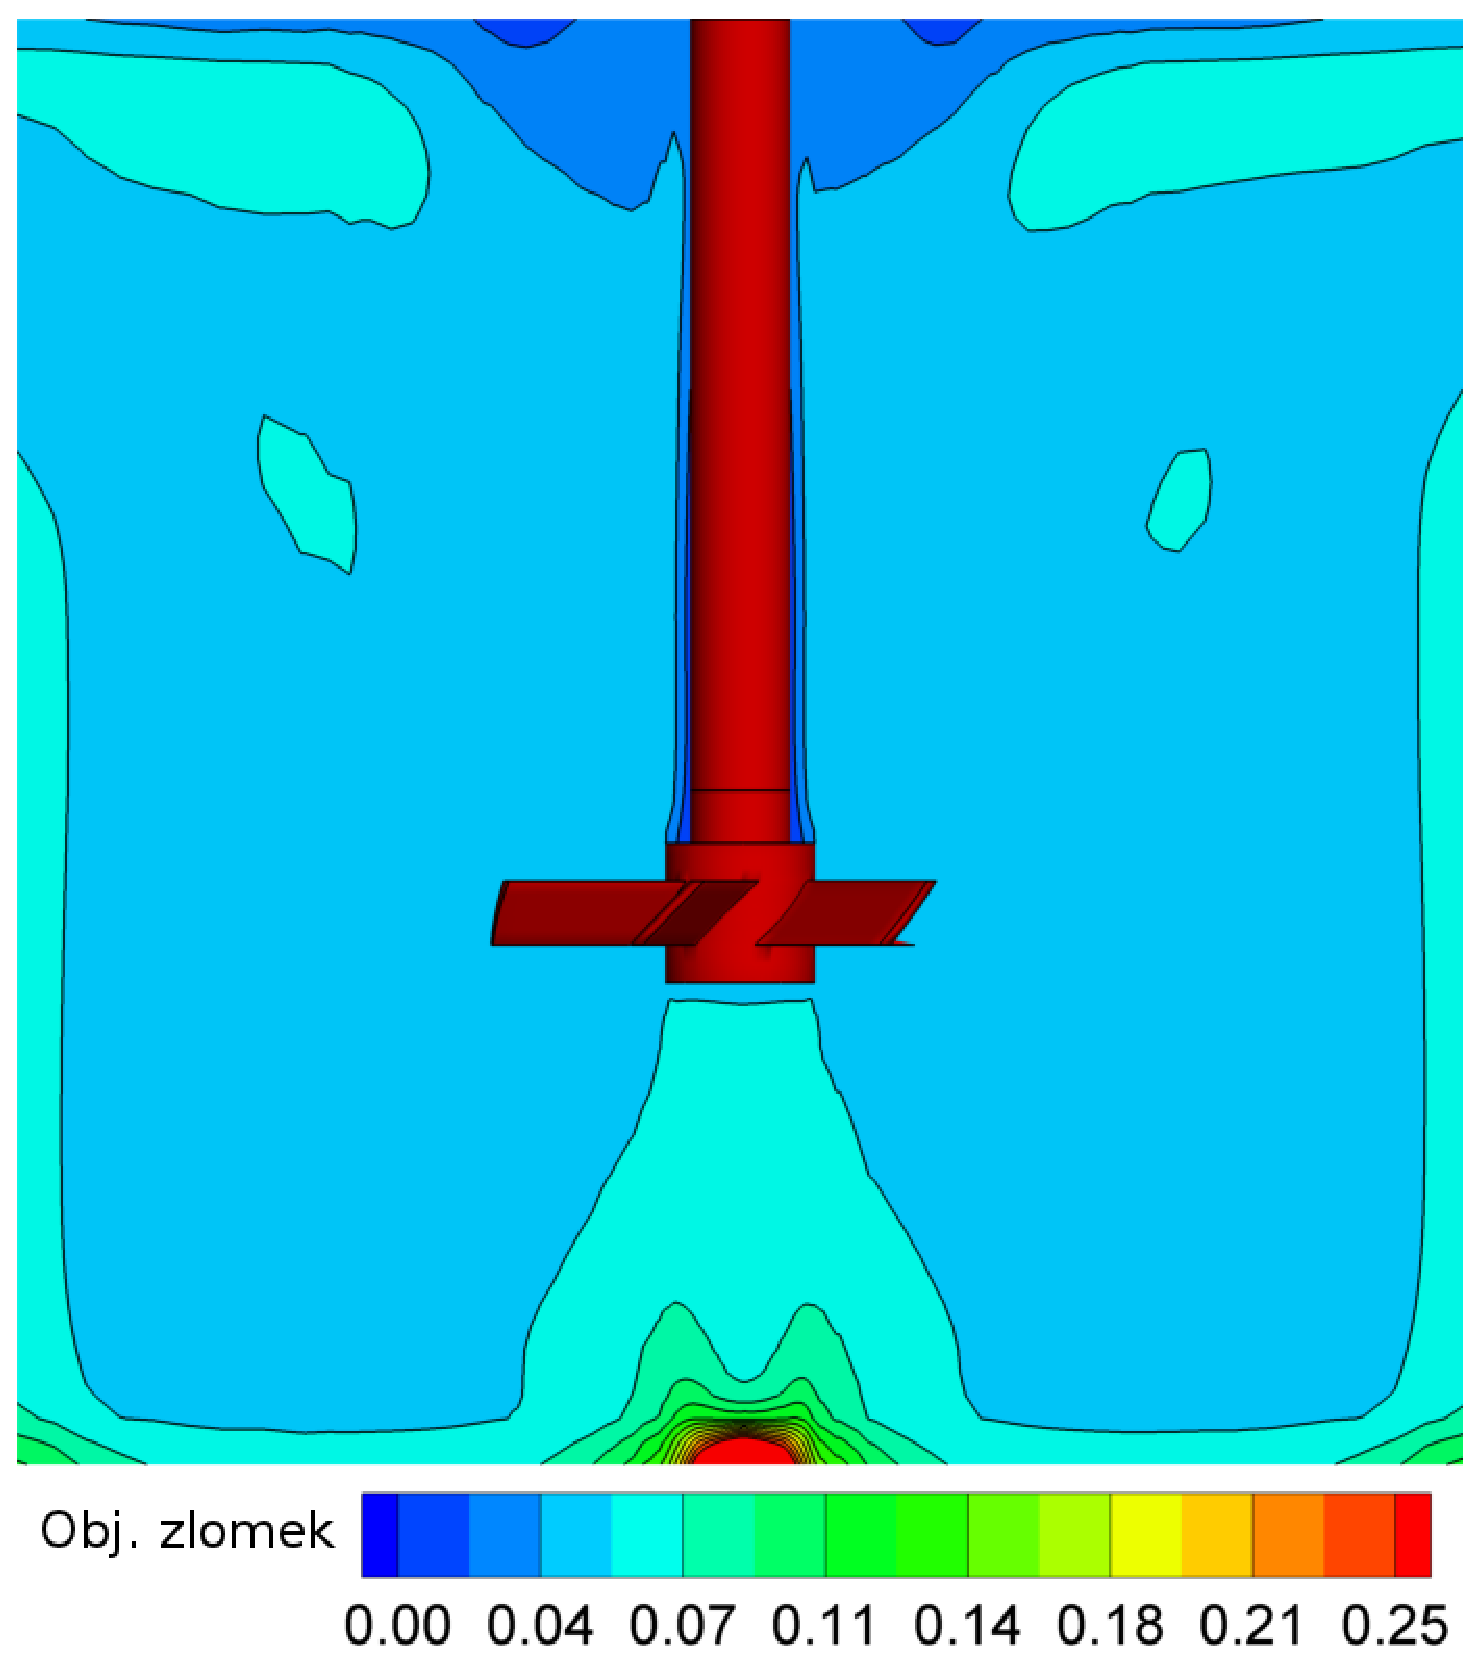
\includegraphics[scale=0.3]{images/volBru-6.eps}}
  \qquad
  \subfloat[Khopkar]{\label{fig:kho6}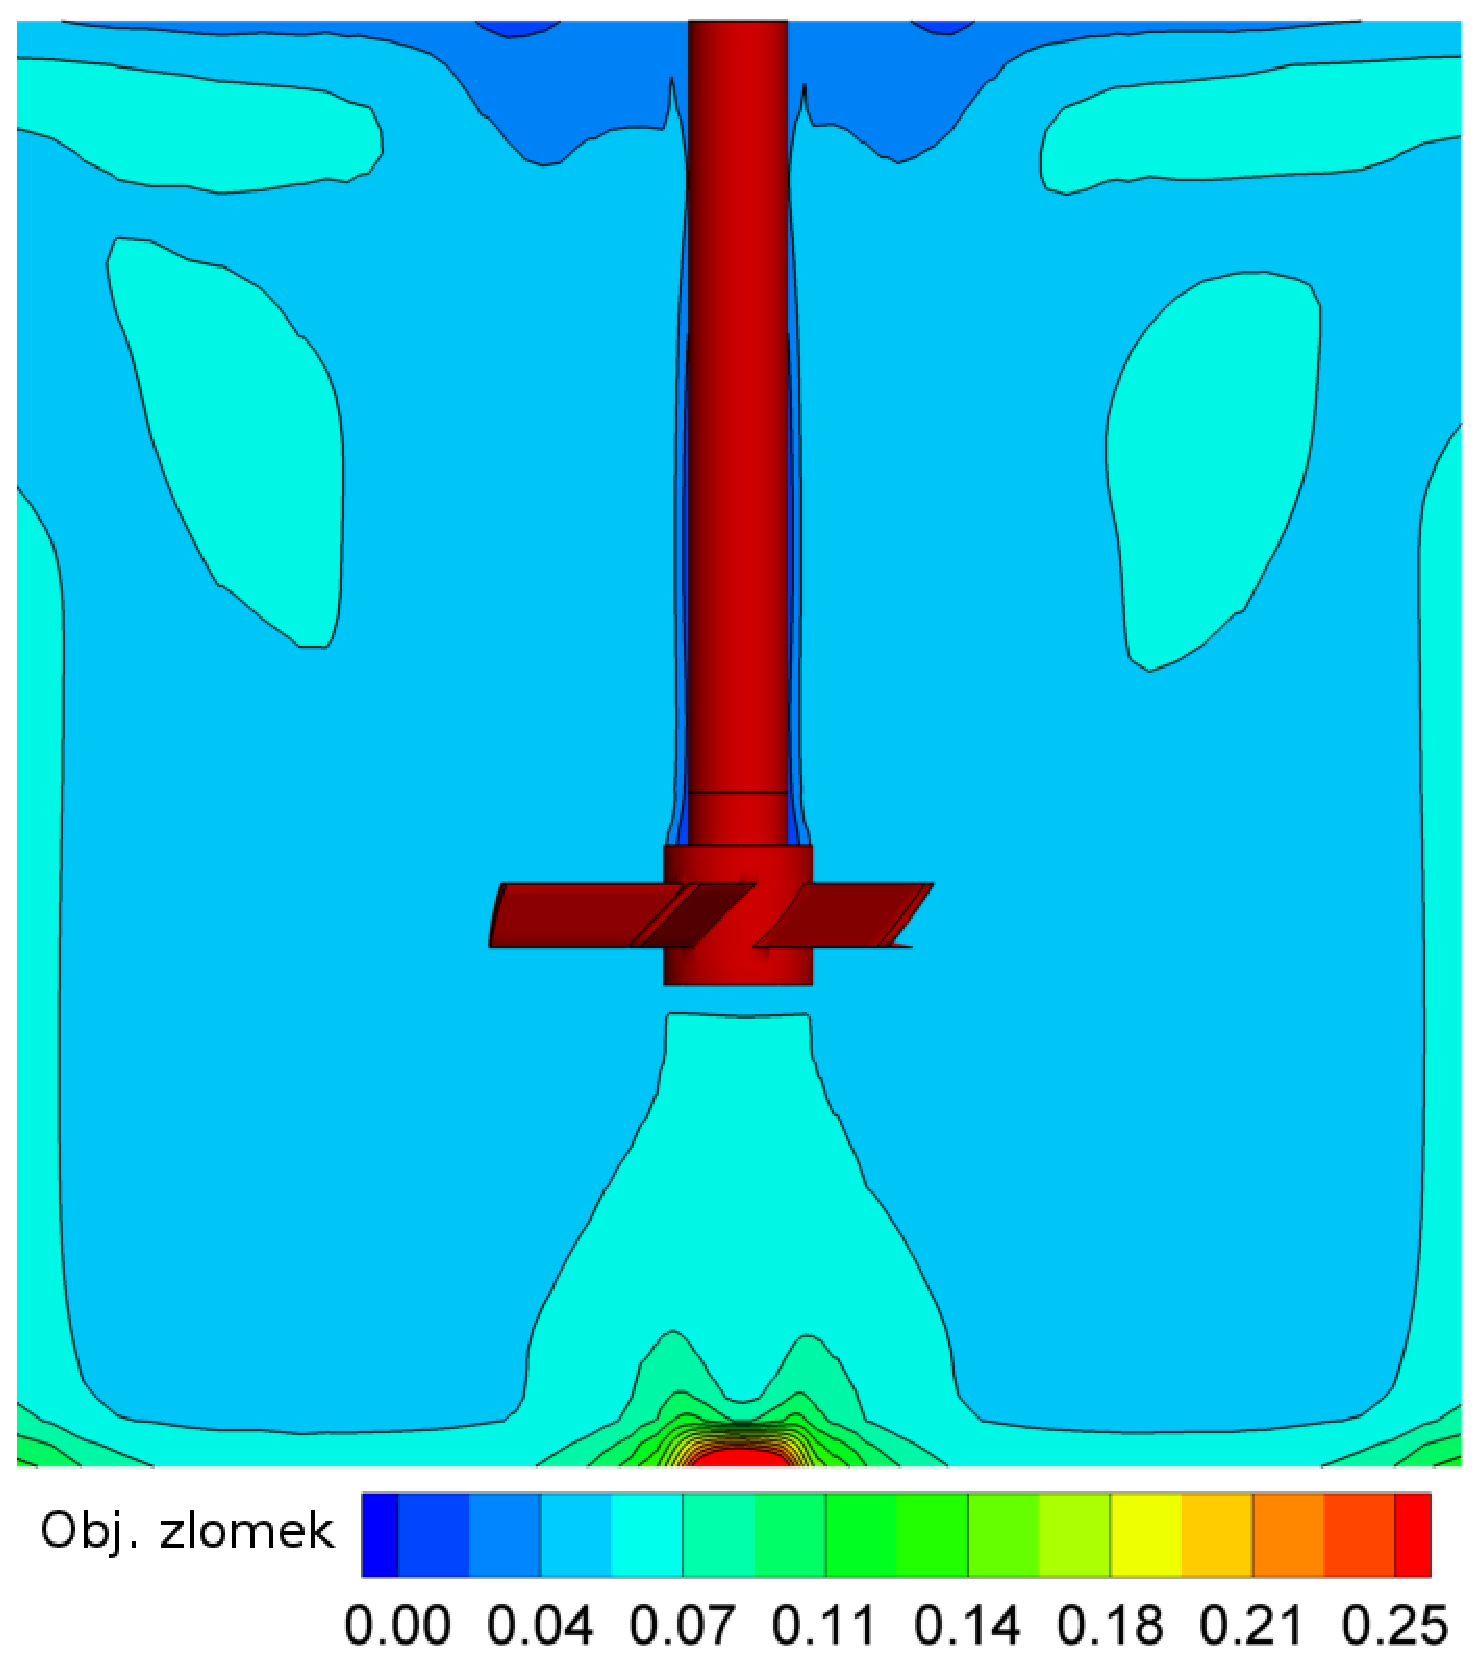
\includegraphics[scale=0.3]{images/volKho-6.eps}}
  \caption{Kocentrace pevné fáze v čase \SI{6}{\second}}
  \label{fig:count6}
  \end{center}
\end{figure}

\vspace{-9mm}

Následují grafické závislosti odporového koeficientu 

\newpage

\begin{figure}[h!]
\begin{center}
\includegraphics[scale=0.47]{images/Vol-2.eps}
\caption{Vektorové pole rychlosti}
\label{fig:vol2}
\end{center}
\end{figure} 

\vspace{-12mm}

\begin{figure}[h!]
\begin{center}
\includegraphics[scale=0.47]{images/Vol-6.eps}
\caption{Vektorové pole rychlosti}
\label{fig:vol6}
\end{center}
\end{figure} 

\vspace{-9mm}

Následují grafické závislosti odporového koeficientu 

\newpage

\begin{figure}[h!]
\begin{center}
\includegraphics[scale=0.47]{images/CD-2.eps}
\caption{Vektorové pole rychlosti}
\label{fig:cd2}
\end{center}
\end{figure} 

\vspace{-12mm}

\begin{figure}[h!]
\begin{center}
\includegraphics[scale=0.47]{images/CD-6.eps}
\caption{Vektorové pole rychlosti}
\label{fig:cd6}
\end{center}
\end{figure} 

\vspace{-9mm}

Následují grafické závislosti odporového koeficientu 


  \chapter{Závěr}
Následující práce byla zaměřena na posouzení vlivu použitého modelu pro koeficient odporu na výsledky CFD simulace suspendace v~mechanicky míchané nádobě. V~rámci této studie bylo implementováno několik korelací pro koeficient odporu v~turbulentní oblasti proudění pomocí uživatelsky definovaných funkcí. Pomocí techniky CFD bylo simulováno promíchávání pevné fáze o~koncentraci 5\,\%\,obj. ve vsádce polyvinylpyrrolidonu.

Ze získaných výsledků vyplynulo, že daný model pro koeficient odporu ovliňuje distribuci pevné fáze zvláště při vyšších objemových zlomcích dané fáze. Tento fakt dobře ilustruje obr. \ref{fig:vol2}. Model navržený \hyperlink{hyp:cds}{Brucatem} pro Taylorův–Couetteovův tok vykazoval ve všech případech výrazně odlišné chování, a proto ho nelze doporučit pro simulaci suspendaci v~mechanicky míchané nádobě. Zbývající modely projevovaly velmi podobné chování, co se týče výsledných koncentračních profilů. 

Budoucí výzkum se zaměří na stanovení výšky vznosu pevné fáze spolu s~určením doby homogenizace a porovnáním s~dostupnými experimentálními výsledky. CFD simulace bude provedena i pro vyšší objemové zlomky pevné fáze spolu se srovnáním dalších vícefázových modelů (např. \nameref{sec:egm}).  


  \chapter*{Seznam symbolů}
\addcontentsline{toc}{chapter}{Seznam symbolů}

\renewcommand\arraystretch{1.5}
\begin{tabularx}{\textwidth}{@{}p{1.0cm} X r@{}}
	$b$ & šířka narážky & \si{\meter} \\
	$c$ & koncentrace & \si{\mole\per\cubic\meter} \\
	$c^{*}$ & bezrozměrná koncentrace & --\\
	$C$ & vzdálenost míchadla ode dna nádoby & \si{\meter} \\
	$C_{D0}$ & odporový koeficient podle Schillera-Naumanna & -- \\ 
	$C_{D}$ & odporový koeficient &  -- \\
	$d_{s}$ & průměr částice & \si{\meter} \\
	$D$ & průměr míchadla & \si{\meter} \\
	
	$\vec{f}_{ext}$ & objemová síla působící na objemový element & \si{\newton\per\cubic\meter} \\
	$\vec{f}_{int}$ & povrchová síla působící na objemový element & \si{\newton\per\cubic\meter} \\
	$\vec{F}_{ad}$ & další síly & \si{\newton} \\
	$\vec{F}_{D}$ & odporová síla & \si{\newton} \\
	$\vec{F}_{g}$ & gravitační síla & \si{\newton} \\
	$\vec{F}_{vz}$ & vztlaková síla & \si{\newton} \\
	$\vec{g}$ & gravitační zrychlení & \si{\meter\per\second\squared} \\
	$H$ & výška plnění nádoby & \si{\meter} \\
	$K$ & koeficient mezifázového sdílení hybnosti & \si{\kilogram\per\cubic\meter\per\second} \\
	$m_{p}$ & hmotnost částice & \si{\kilogram} \\
	
	$p$ & tlak & \si{\pascal} \\
	$\vec{R}$ & mezifázová odporová síla působící na objemový element & \si{\newton\per\cubic\meter} \\
	$Re_{p}$ & Reynoldsovo kritérium pro pevnou částici &  --\\
	$t$ & čas & \si{\second} \\
	$T$ & vnitřní průměr nádoby & \si{\meter} \\
	$U$ & napětí & \si{\volt} \\
	$\vec{v}_{p}$ & rychlost & \si{\meter\per\second} \\
\end{tabularx}


\subsubsection*{Řecké symboly}
\begin{tabularx}{\textwidth}{@{}p{1.0cm} X r@{}}
$\alpha$ & objemový zlomek& --\\
$\eta$ & dynamická viskozita & \si{\pascal\second} \\
$\lambda$ & Kolmogorovo mikroměřítko  & \si{\meter} \\
$\rho$ & hustota & \si{\kilogram\per\cubic\meter} \\
$\bar{\tau}$ & deviátor tenzoru napětí& \si{\pascal} \\
\end{tabularx}

\subsubsection*{Spodní indexy}
\begin{tabularx}{\textwidth}{@{}p{1.0cm} X r@{}}
$f$ & tekutina & \\
$i$ & $i$-tá fáze & \\
$j$ & $j$-tá fáze & \\
$p$ & pevná částice & \\
$s$ & pevná fáze & \\
\end{tabularx}


\subsubsection*{Zkratky}
\begin{tabularx}{\textwidth}{@{}p{1.0cm} X }
CFD & computational fluid dynamics  \\
PVC & polyvinylchlorid  \\
PVP & polyvinylpyrrolidon  \\
UDF & user defined function  \\
\end{tabularx}

	\normalsize{}
	%\setlength{\bibhang}{0pt} odsazen prvního řádku bibliografie
	\begin{thebibliography}{99}
\addcontentsline{toc}{chapter}{Bibliography}

\bibitem[Armenante \textit{et al.}, 1998]{arm98} Armenante, P. M., Nagamine, E. U., Susanto, J., 1998. Determination of correlations to predict the minimum agitation speed for complete solid suspension in agitated vessels. \textit{Can J Chem Eng}, \textbf{76}, 413--419

\bibitem[Baldi \textit{et al.}, 1978]{bal78} Baldi, G., Conti, R., Alaria, E., 1978. Complete suspension of particles in mechanically agitated vessels. \textit{Chem Eng Sci}, \textbf{33}, 21--25 

\bibitem[Brucato \textit{et al.}, 1998]{bru98} Brucato, A., Grisafi, F., Montante, G., 1998. Particle drag coefficients in turbulent fluids. \textit{Chem Eng Sci}, \textbf{43}, 3, 3295--3314

\bibitem[Derksen, 2003]{derk03} Derksen, J.J., 2003. Numerical Simulation of solid suspension in a stirredtank. \textit{AIChE J}, \textbf{49}, 11, 2700--2714

\bibitem[Ihme \textit{et al.}, 1972]{ihme72} Ihme, F., Schmidt-Traub H., Brauer, H., 1972. Theoretische untersuchung \"uber die Umstr\"omung und den Stoff\"ubergang an Kugeln. \textit{Chem.-Ing.-Tech.}, \textbf{44}, 306

\bibitem[Ishii-Zuber, 1979]{ish79} Ishii, M., Zuber, N., 1979, Drag coefficient and relative velocity in bubbly, droplet or particulate flows, \textit{AIChE J}, \textbf{28}, 843--855 

\bibitem[Kresta and Wood, 1991]{kre91} Kresta, S. M., Wood, P. E., 1991. Prediction of three-dimensional turbulent flow in stirred tanks. \textit{AIChE J}, \textbf{37}, 448--460 

\bibitem[Ljungqvist and Rasmuson, 2001]{lju01} Ljungqvist, M., Rasmuson, A., 2001. Numerical simulation of the two-phase flow in an axially stirred reactor. \textit{Trans AIChE}, \textbf{79}, Part A, 533--546

\bibitem[Micheletti \textit{et al.}, 2003]{miche03} Micheletti, L., Nikiforaki, L., Lee, K.C., Yianeeskis, M., 2003. Integral and Local Concentration Characteristics of Moderate to Dense Solid-Liquid Suspensions. \textit{11$^{th}$ European Conference on Mixing}, Bamberg, Germany


\bibitem[e.g.\ Nienow, 1968]{nie68} Nienow, A. W., 1968. Suspension of solid particles in turbine agitated baffled vessels. \textit{Chem Eng Sci}, \textbf{23}, 1453--1459 

\bibitem[Oshinowo and Bakker, 2001]{oshi02} Oshinowo, L. M., Bakker, A., 2002. CFD modeling of solids suspensions in stirred tanks. \textit{Symposium on Computational Modeling of Metals, Minerals and Materials}, February 17-21, Seattle, Washington 

\bibitem[Schiller-Naumann, 1935]{schi32} Schiller, L., Naumann, Z., 1935. A drag coefficient correlation. \textit{Z. Ver. Deutsch. Ing.}, \textbf{77}, 318--320

\bibitem[Syamlal and O'Brien, 1993]{syam93} Syamlal, M., O'Brien, T.J., 1993. MFIX Documentation: Theory Guide. \textit{National Technical Information Service}, \textbf{1}, Springfield, Virginia 

\bibitem[Zwietering, 1957]{zwi58} Zwietering, T. N., 1958. Suspending of solid particles in liquid by agitators. \textit{Chem Eng Sci}, \textbf{8}, 244--253 

\end{thebibliography}

  \include{priloha}
  
\end{document}
